%    Documentation for PRU ADC Project
%    Copyright (C) 2016  Gregory Raven
%
%    This program is free software: you can redistribute it and/or modify
%    it under the terms of the GNU General Public License as published by
%    the Free Software Foundation, either version 3 of the License, or
%    (at your option) any later version.
%
%    This program is distributed in the hope that it will be useful,
%    but WITHOUT ANY WARRANTY; without even the implied warranty of
%    MERCHANTABILITY or FITNESS FOR A PARTICULAR PURPOSE.  See the
%    GNU General Public License for more details.
%
%    You should have received a copy of the GNU General Public License
%    along with this program.  If not, see <http://www.gnu.org/licenses/>.

\documentclass[oneside,letterpaper,12pt]{book}
\usepackage[utf8]{inputenc}
\usepackage[T1]{fontenc}
\usepackage[top=0.8874in,bottom=0.8874in,left=0.7874in,right=0.7874in]{geometry}
\usepackage{charter}
\usepackage{color}
\usepackage{array,ragged2e}
\usepackage{graphicx}
\usepackage[colorlinks=true, linkcolor=red]{hyperref}
\usepackage{amsmath}
\usepackage{titling,lipsum}
\usepackage{booktabs}
\usepackage{longtable}

\title{This is title of my document}

\begin{document}
{\centering\bfseries\color{black}\Huge
Using the Beaglebone Black Programmable Real-Time Unit with the RemoteProc and Remote Messaging Framework to Capture and Play Data from an ADC
\par}

\bigskip

\begin{figure}
	\centering
	%\includegraphics[width=0.8\textwidth]{rodinialite.png}
	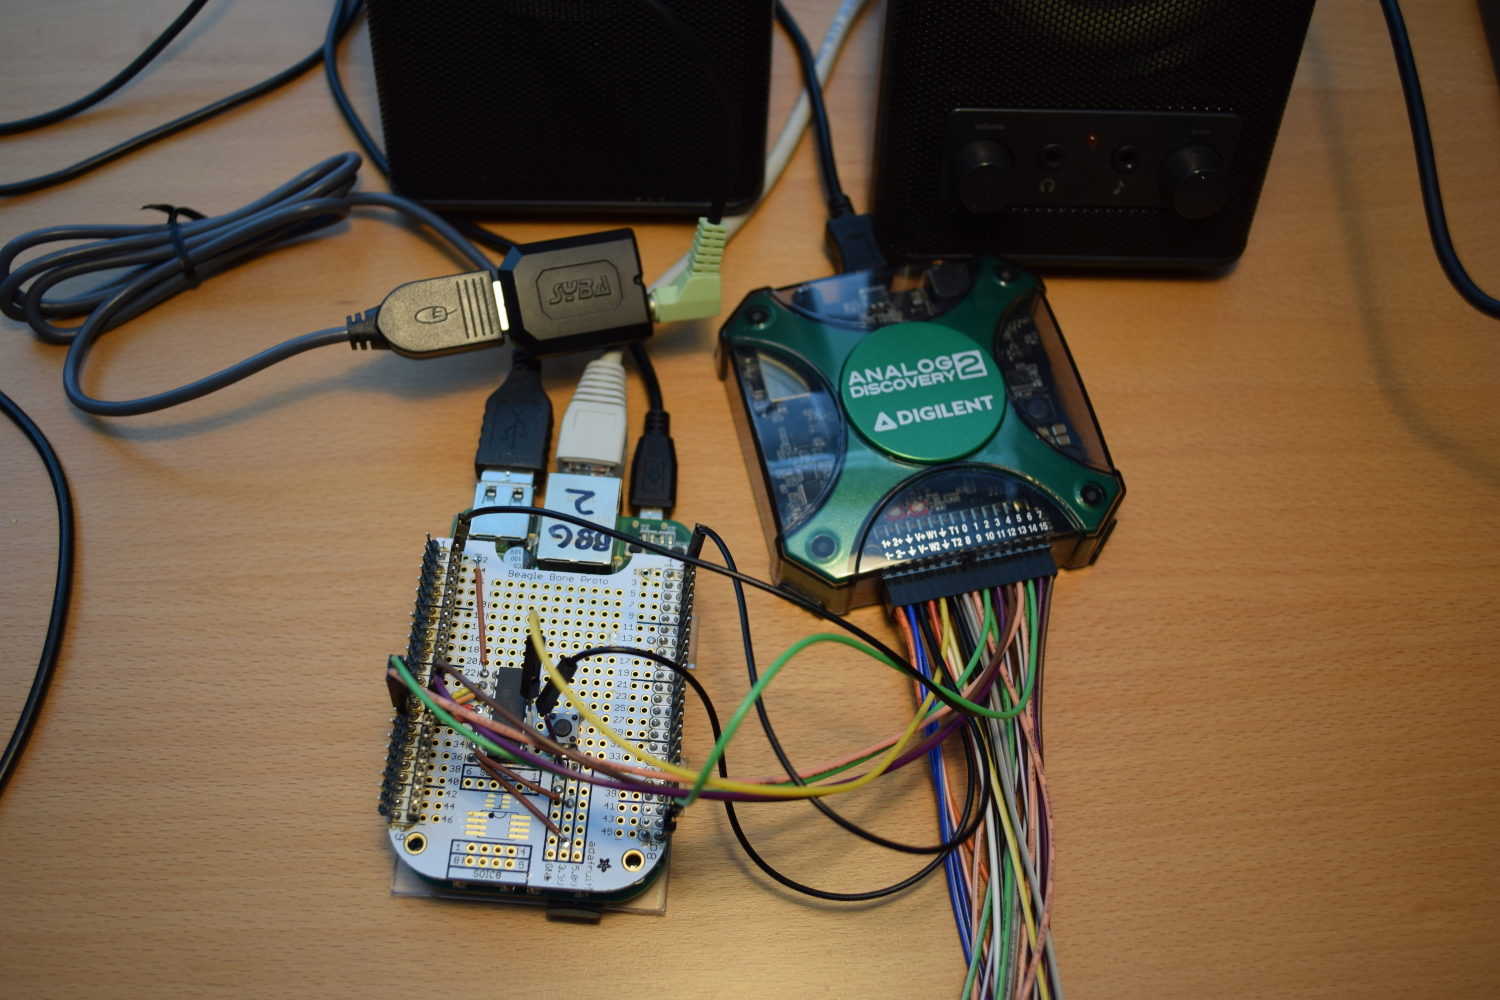
\includegraphics[width=0.8\textwidth]{photos/DSC_0021}
\end{figure}

\bigskip
{\centering\bfseries\Large
Gregory Raven
\par}


\bigskip
{\centering\bfseries\LARGE
October 9, 2016
\par}
\newpage





%\setcounter{page}{1}

%\author{Gregory Raven}
%\title{Using the Beaglebone Black Programmable Real-Time Unit with the RemoteProc %and %Remote Messaging Framework to Capture and Play Data from an ADC}
%\date{October 2016}

%
\frontmatter

%\maketitle
\tableofcontents
\listoftables
\listoffigures
%\maketitle

\mainmatter
%    Documentation for PRU ADC Project
%    Copyright (C) 2016  Gregory Raven
%
%    This program is free software: you can redistribute it and/or modify
%    it under the terms of the GNU General Public License as published by
%    the Free Software Foundation, either version 3 of the License, or
%    (at your option) any later version.
%
%    This program is distributed in the hope that it will be useful,
%    but WITHOUT ANY WARRANTY; without even the implied warranty of
%    MERCHANTABILITY or FITNESS FOR A PARTICULAR PURPOSE.  See the
%    GNU General Public License for more details.
%
%    You should have received a copy of the GNU General Public License
%    along with this program.  If not, see <http://www.gnu.org/licenses/>.

\chapter{Introduction}

This is the documentation for a small embedded GNU/Linux project utilizing the RemoteProc and RPMsg framework in the Beaglebone Green (BBG) development board.  The project repository is located here:

\url{https://github.com/Greg-R/pruadc1}

The inspiration for this project came from the superb book ``Exploring Beaglebone'' by Derek Molloy.  Professor Molloy's project utilized assembly code and the UIO driver.  The hardware used in this project is essentially a copy of the Molloy design.

Recent developments in the Texas Instruments PRU support include the RemoteProc and Remote Messaging frameworks, as well as an extensively documented C compiler and much additional supporting documentation.  This project utilizes these frameworks and is entirely dependent upon C code in both the PRU and GNU/Linux user space.  The detailed examples provided by TI in the ``PRU Support Package'' were invaluable in developing this project:

\url{https://git.ti.com/pru-software-support-package}

A listing of additional resources is found in the Resources chapter.

An MCP3008 Analog-to-Digital Converter (ADC) IC is connected to the BBG GPIO pins which are in turn connected to the PRU using the ``Universal IO'' kernel driver which is deployed by default to the current distributions of Debian on the Beaglebones.  The PRUs communicate with a user-space C program via ``character devices'' created by the remote messaging kernel driver.  The data is pushed to a USB codec via the ``Advanced Linux Sound Architecture'', and finally, to an analog speaker.  The diagram below illustrates the flow of data through the system.


\begin{figure}[H]
	\centering
	\includegraphics[width=0.8\textwidth]{diagrams/data_flow_intro}
	\centering\bfseries
	\caption{Flow of Data Through the System}
\end{figure}

\section{Project Goals}

This project does not solve a specific practical problem.  It is a laboratory experiment.

The primary goal is to learn to program the PRUs, and to control and communicate with them from the operating system's ``user space''.  Here is a list of the project goals and sub-goals:

\begin{itemize}
	\item Write C code for the PRUs which implement a SPI bus.
	\item Build a ``proto-cape'' with an ADC.
	\item Use the ``Universal IO'' to configure the PRU interface to the GPIO pins.
	\item Write a user-space C program which communicates with the PRUs via character devices.
	\item Use the Analog Discovery 2 as a logic analyzer to debug the PRU SPI C code.
	\item Stream the digitized audio data from the ADC to the ``Advanced Linux Sound Architecture'' in real time.  Play the audio to a speaker.
	\item Document and publish the project to Github.
\end{itemize}

\section{Limitations}

The BeagleBone's Sitara ``System On Chip'' is quite powerful, and this power is probably masking several inefficiencies in the project's design.  All of the testing and debugging was done with a bare-bones Debian distribution with no other significant processes running.

The speaker audio does not have noticeable distortion or glitches when listening with the speaker.  The audio was not examined with a spectrum or distortion analyzer.  It may not be the best quality audio.

The audio sample rate was limited to 8 kHz, which is the lowest rate accepted by ALSA.  A follow-up investigation will see if the sample rate can be increased.  It is not known what aspect of the system will begin to break down as sample rate is increased.

The sample rate had to be ``tuned'' to prevent ``buffer underruns'' reported by the ALSA system.  An approach to make the real-time data stream robust is not known by the author and needs further investigation.

All of the development was done as root user via ssh on the BeagleBone Green.  This is generally not a good practice, however, considering this as an embedded and experimental project it was not considered to be a serious drawback.



%    Documentation for PRU ADC Project
%    Copyright (C) 2016  Gregory Raven
%
%    This program is free software: you can redistribute it and/or modify
%    it under the terms of the GNU General Public License as published by
%    the Free Software Foundation, either version 3 of the License, or
%    (at your option) any later version.
%
%    This program is distributed in the hope that it will be useful,
%    but WITHOUT ANY WARRANTY; without even the implied warranty of
%    MERCHANTABILITY or FITNESS FOR A PARTICULAR PURPOSE.  See the
%    GNU General Public License for more details.
%
%    You should have received a copy of the GNU General Public License
%    along with this program.  If not, see <http://www.gnu.org/licenses/>.

\chapter{System Diagram}


\begin{figure}[h]
\centering
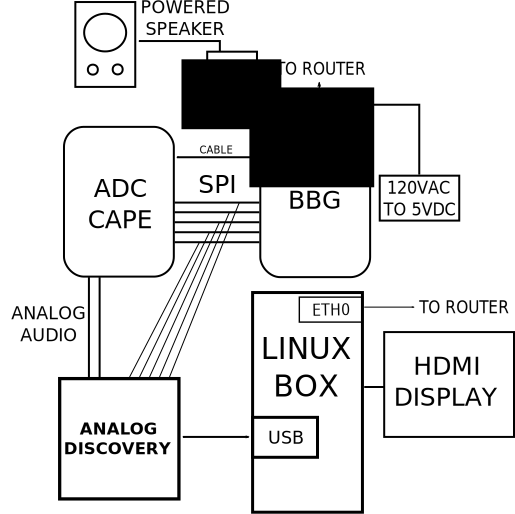
\includegraphics[width=0.8\textwidth]{diagrams/system_ink}
\centering\bfseries
\caption{PRU-ADC System Diagram}
\end{figure}

The system diagram as shown includes all of the facilities used during development.

The ``Linux Box'' is a desktop PC architecture machine running Ubuntu 14.04/16.04.  Communication to the BBG was done via ``Secure Shell'' (SSH).  The Linux Box also served as host for the Analog Discovery 2 and GUI via the HDMI display.  The Analog Discovery 2 also provided analog audio to the ADC input.

The ``Beagle Bone Green'' (BBG) is the TI Sitara-based platform board manufactured by Seeed Studio.

The ``ADC Cape'' is an Adafruit breadboard with the MCP3008 and headers soldered to it.  A few wires are required to complete the connections to the ADC to the header pins, DC bias and ground.

The ``USB Codec'' plugs into the USB connector on the BBG.  Due to interference with the adjacent ethernet connector, a short USB extension cable is recommended.





%    Documentation for PRU ADC Project
%    Copyright (C) 2016  Gregory Raven
%
%    This program is free software: you can redistribute it and/or modify
%    it under the terms of the GNU General Public License as published by
%    the Free Software Foundation, either version 3 of the License, or
%    (at your option) any later version.
%
%    This program is distributed in the hope that it will be useful,
%    but WITHOUT ANY WARRANTY; without even the implied warranty of
%    MERCHANTABILITY or FITNESS FOR A PARTICULAR PURPOSE.  See the
%    GNU General Public License for more details.
%
%    You should have received a copy of the GNU General Public License
%    along with this program.  If not, see <http://www.gnu.org/licenses/>.

\chapter{Prototype Cape Detail}




The proto-cape schematic is simple, and is composed of a single component, the MCP3008 ADC.

\begin{figure}[H]
	\centering
	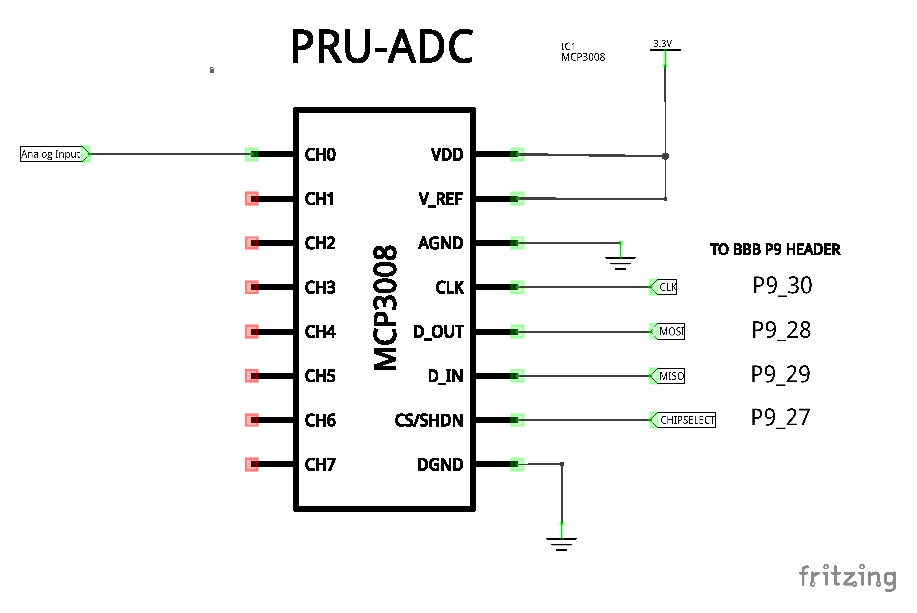
\includegraphics{../../pcb/pru_adc_schematic_schem}
	\centering\bfseries
	\caption{PRU-ADC Cape Breadboard}
\end{figure}

The ``Cape'' was built on an Adafruit proto-cape:

\url{https://www.adafruit.com/products/572}

Here is a breadboard diagram from Fritzing which shows how the proto-cape
is wired:

\begin{figure}[H]
	\centering
	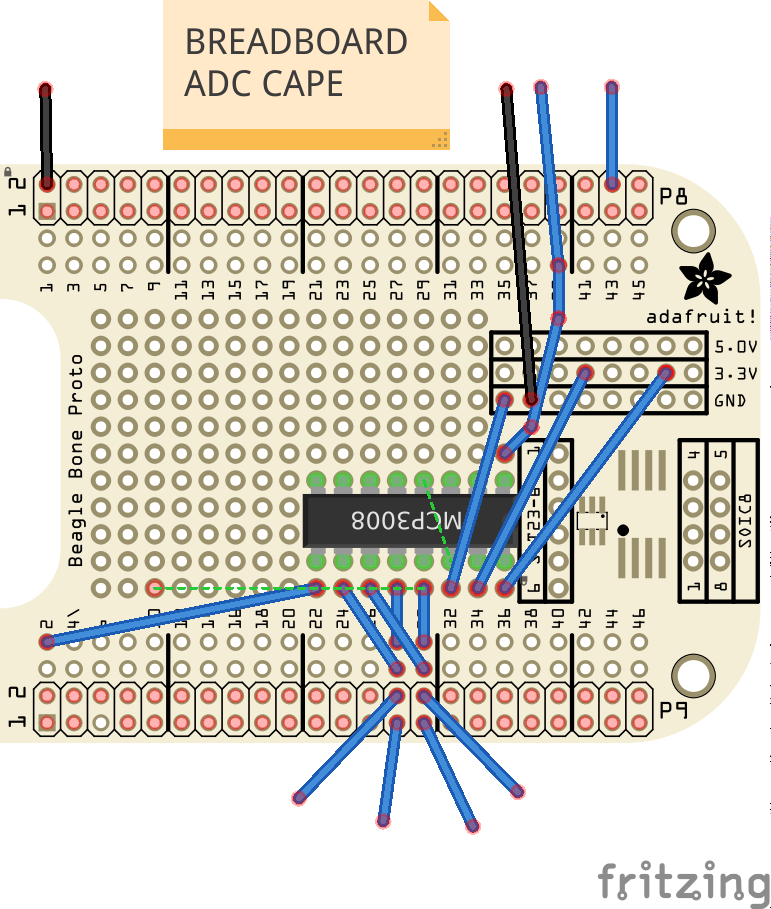
\includegraphics[]{../../pcb/adafruit_proto_cape_bb}
	\centering\bfseries
	\caption{PRU-ADC Cape Breadboard}
\end{figure}

In addition to the header pins required to plug into the BBB, extra rows of headers were soldered to the top of the breadboard.  This allows easy connection to the Discovery Analog 2 as seen in the following photograph.

\begin{figure}[H]
	\centering
	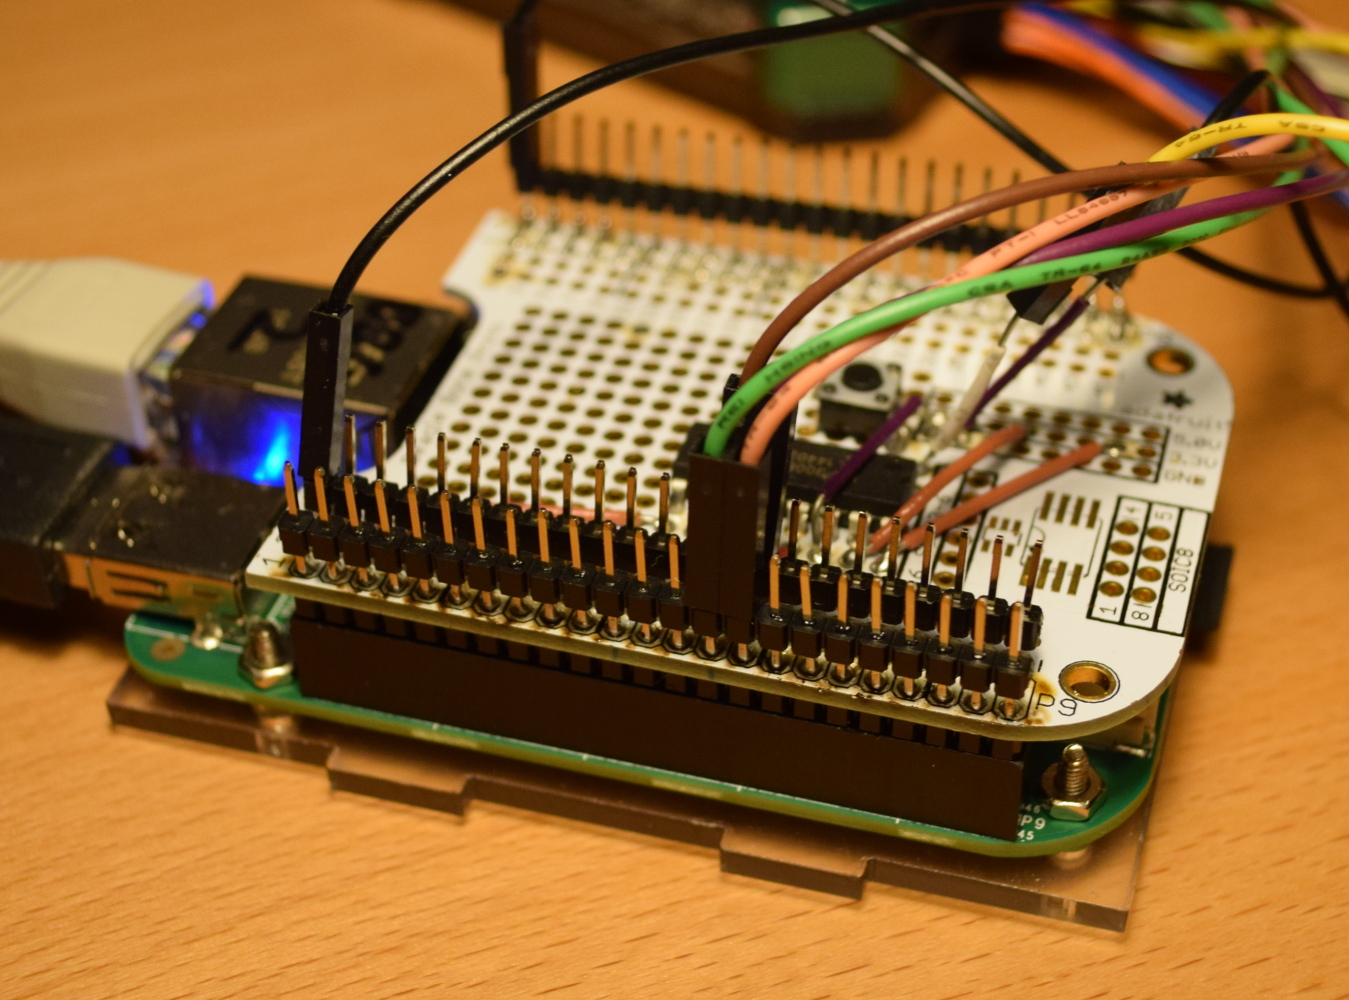
\includegraphics{photos/DSC_0025}
	\centering\bfseries
	\caption{PRU-ADC Cape Breadboard}
\end{figure}


%    Documentation for PRU ADC Project
%    Copyright (C) 2016  Gregory Raven
%
%    This program is free software: you can redistribute it and/or modify
%    it under the terms of the GNU General Public License as published by
%    the Free Software Foundation, either version 3 of the License, or
%    (at your option) any later version.
%
%    This program is distributed in the hope that it will be useful,
%    but WITHOUT ANY WARRANTY; without even the implied warranty of
%    MERCHANTABILITY or FITNESS FOR A PARTICULAR PURPOSE.  See the
%    GNU General Public License for more details.
%
%    You should have received a copy of the GNU General Public License
%    along with this program.  If not, see <http://www.gnu.org/licenses/>.

\chapter{PRU Firmware and User-space Program}

The ``PRU Firmware'' are two binary files which are placed in the directory /lib/firmware.
These files must have specific names as follows:

\begin{itemize}
	\item am335x-pru0-fw
	\item am335x-pru1-fw
\end{itemize}

The Makefile includes cp commands to copy the firmwares to the /lib/firmware directory.

\section{Implementing the SPI Bus in C}

The SPI bus C program roughly follows the PRU assembly code written by Derek Molloy.  The C code is compiled to a binary file am335x-pru0-fw. The firmware is loaded into PRU0 automatically by the remoteproc kernel driver.

The program begins with code sequestered from the example code files in TI's PRU Software
Support Package.  This codes establishes the character device driver via the ``Remote Proc Messenger''
kernel driver.  There is a sort of ``priming'' process required whereby a user space program writes
to the device driver.  The initializes the character driver, which allows it to write data from
the PRU to the character driver and thus making the data available in user-space.

After the initialization is complete, the program enters a for loop.  The SPI bus is implemented inside this for loop.  This is done by bit-banging the GPIOs which have been connected to PRU0 via the Universal IO.  Each pass through the for loop captures a single 10-bit sample from the ADC.

The samples are accumulated in a buffer.  When the buffer is filled, the data is written to the character device via a function provided by the RPMsg kernel driver.

Timings are critical, and this was accomplished by using the compiler intrinsic \_\_delay\_cycles.  Each delay is an absolute value of 5 nanoseconds.  This scheme appears to produce accurate enough timing to implement the SPI bus in real time.  

\section{Implementing the Timing Clock in C}

\section{The User-Space Program}


\chapter{Incorporating Advanced Linux Sound Architecture or ``ALSA''}

Pulse Code Modulation
\chapter{RemoteProc Framework and RemoteProc Messaging}


Diagram showing Character Drivers
Data Flow from PRU to ARM

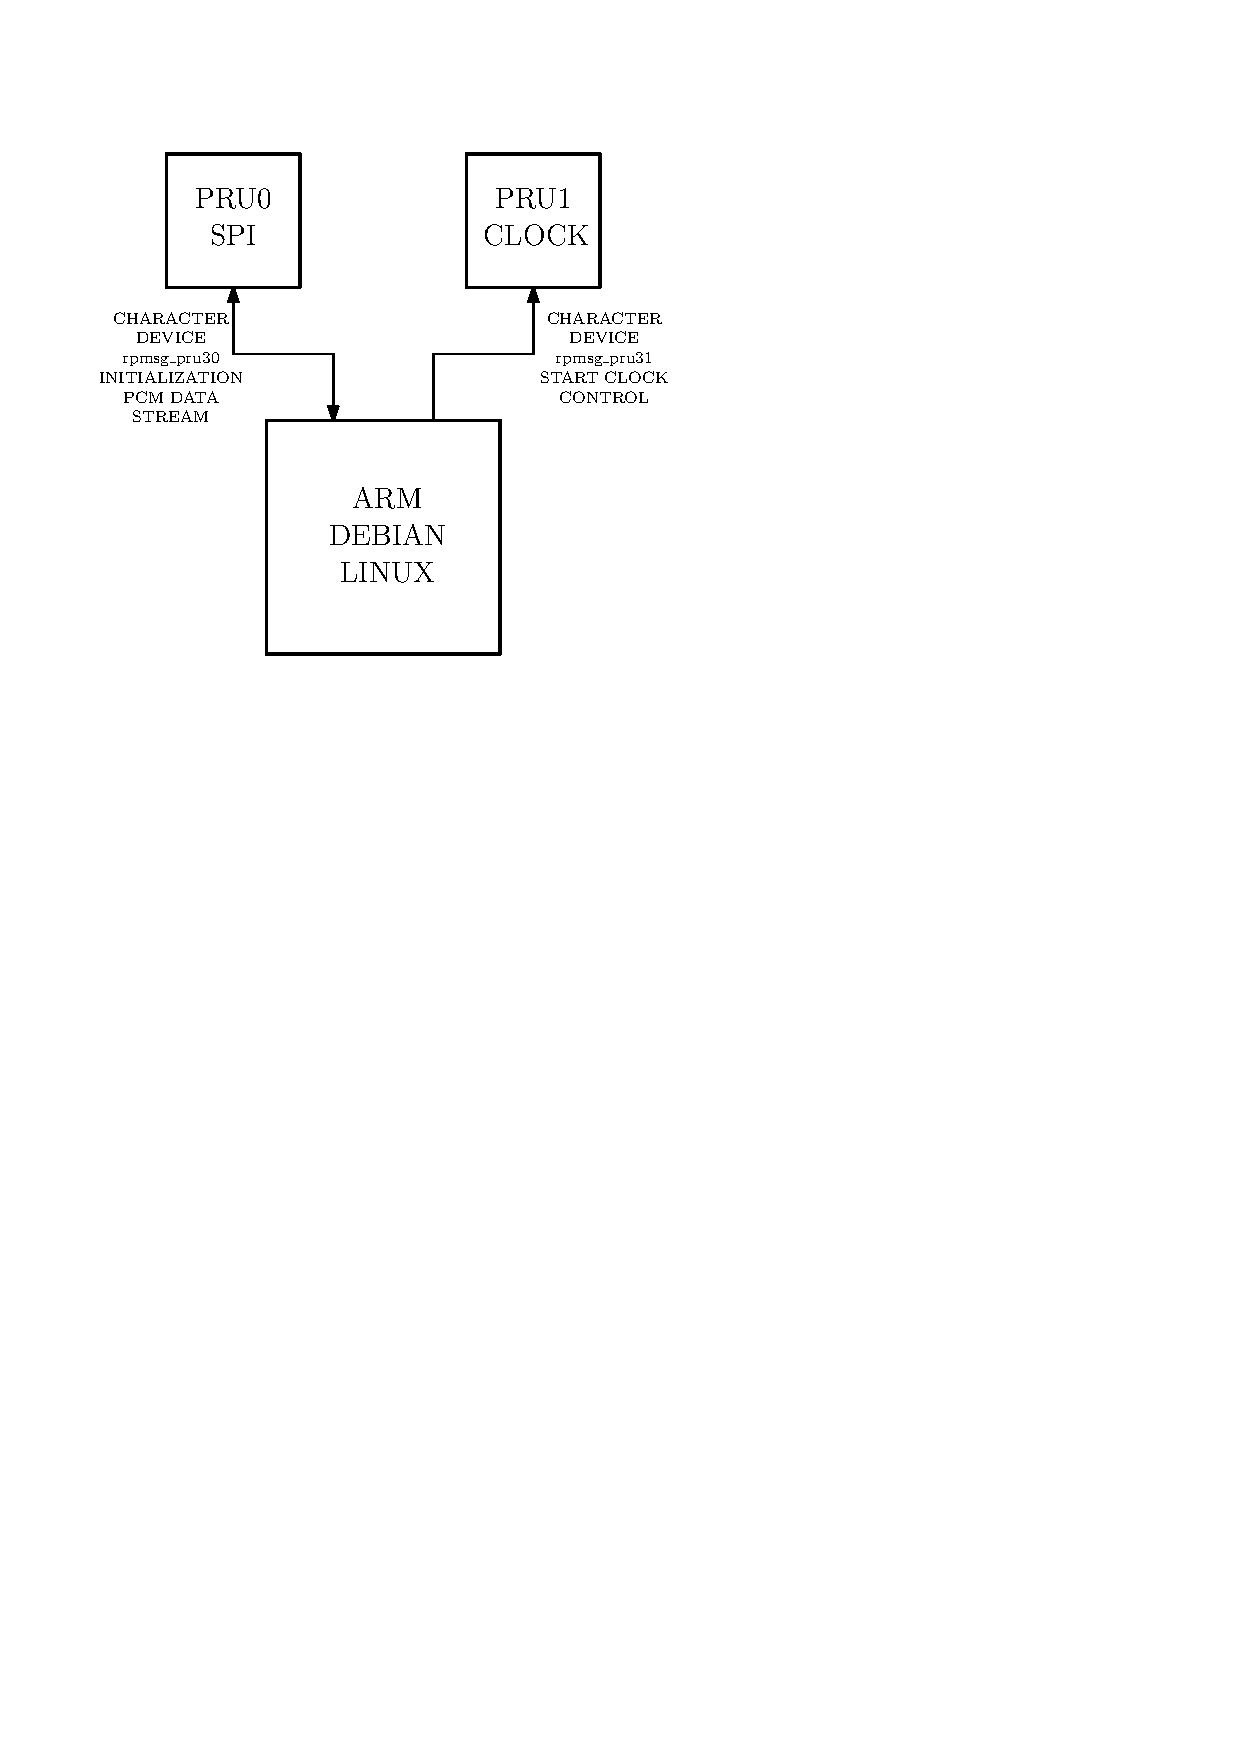
\includegraphics{diagrams/char_devices_2}

Control of the PRU Clock Using Character Driver


%    Documentation for PRU ADC Project
%    Copyright (C) 2016  Gregory Raven
%
%    This program is free software: you can redistribute it and/or modify
%    it under the terms of the GNU General Public License as published by
%    the Free Software Foundation, either version 3 of the License, or
%    (at your option) any later version.
%
%    This program is distributed in the hope that it will be useful,
%    but WITHOUT ANY WARRANTY; without even the implied warranty of
%    MERCHANTABILITY or FITNESS FOR A PARTICULAR PURPOSE.  See the
%    GNU General Public License for more details.
%
%    You should have received a copy of the GNU General Public License
%    along with this program.  If not, see <http://www.gnu.org/licenses/>.

\chapter{Universal IO and Connecting PRU to the Outside World}

This project did not require a custom ``Device Tree Overlay''.  Instead, the ``Universal IO'' driver was used along with a simple shell script.

The Universal IO project is located at this Github repository:

\url{https://github.com/cdsteinkuehler/beaglebone-universal-io}

The configuration is as follows:

\begin{verbatim}
config-pin P8.30 pruout
config-pin P9.31 pruout
config-pin P9.27 pruout
config-pin P9.29 pruout
config-pin P9.28 pruin
config-pin P9.30 pruout
\end{verbatim}

The above can also be put into a file, for example ``pru-config'':

\begin{verbatim}
P8.30 pruout
P9.31 pruout
P9.27 pruout
P9.29 pruout
P9.28 pruin
P9.30 pruout
\end{verbatim}

The command to load the above would be:

config-pin -f pru-config

Note that another step required is create the \$SLOTS environment variable
and also to set on of the Universal-IO device trees as follows:

\begin{verbatim}
export SLOTS=/sys/devices/platform/bone_capemgr
echo univ-emmc > $SLOTS/slots 
\end{verbatim}


\subsection{The PRU GPIO Spreadsheet}

Use ``git clone'' to download this repository:

\url{https://github.com/selsinork/beaglebone-black-pinmux}

The spreadsheet file contained in this repository is pinmux.ods.
The LibreOffice suite has a spreadsheet application which will read
this file.

This spreadsheet is extremely useful when configuring the PRU or
other functions to the Beaglebone pin multiplexer.




\chapter{User Space Program: Fork and Named Pipe}


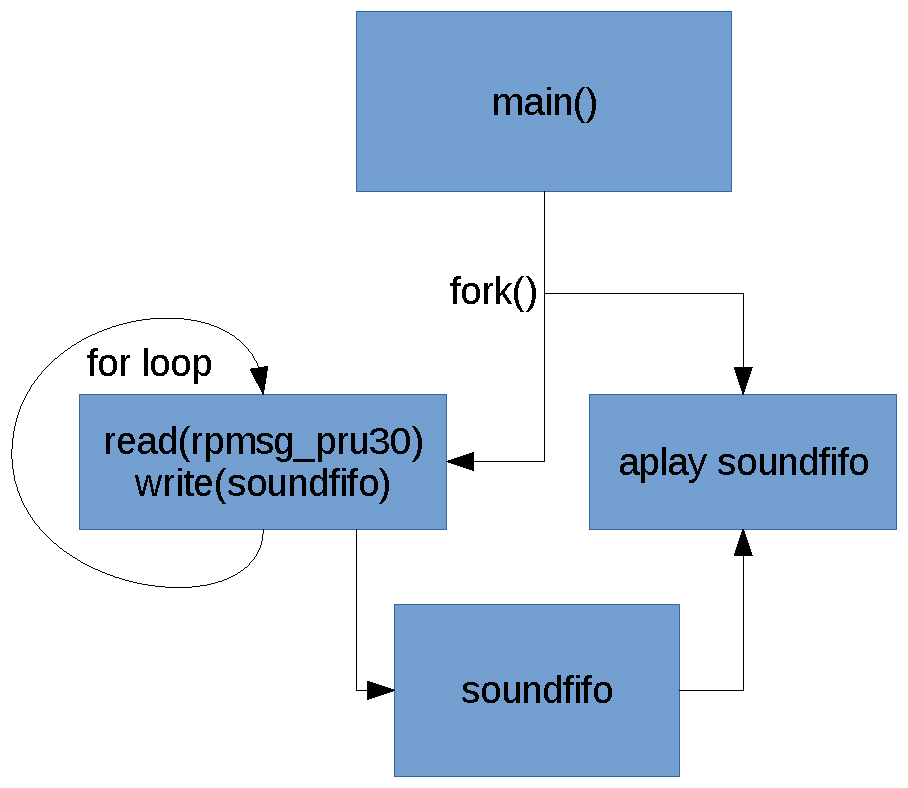
\includegraphics{diagrams/fork-crop}
%    Documentation for PRU ADC Project
%    Copyright (C) 2016  Gregory Raven
%
%    This program is free software: you can redistribute it and/or modify
%    it under the terms of the GNU General Public License as published by
%    the Free Software Foundation, either version 3 of the License, or
%    (at your option) any later version.
%
%    This program is distributed in the hope that it will be useful,
%    but WITHOUT ANY WARRANTY; without even the implied warranty of
%    MERCHANTABILITY or FITNESS FOR A PARTICULAR PURPOSE.  See the
%    GNU General Public License for more details.
%
%    You should have received a copy of the GNU General Public License
%    along with this program.  If not, see <http://www.gnu.org/licenses/>.

\chapter{Shell Scripts}

%    Documentation for PRU ADC Project
%    Copyright (C) 2016  Gregory Raven
%
%    This program is free software: you can redistribute it and/or modify
%    it under the terms of the GNU General Public License as published by
%    the Free Software Foundation, either version 3 of the License, or
%    (at your option) any later version.
%
%    This program is distributed in the hope that it will be useful,
%    but WITHOUT ANY WARRANTY; without even the implied warranty of
%    MERCHANTABILITY or FITNESS FOR A PARTICULAR PURPOSE.  See the
%    GNU General Public License for more details.
%
%    You should have received a copy of the GNU General Public License
%    along with this program.  If not, see <http://www.gnu.org/licenses/>.

\chapter{Setting up the Remoteproc PRU and Compiler on the Beaglebone Green}

The following describes the simplest possible set-up.  Everything was done via the command line, and the vim editor was used extensively to develop the C code and shell scripts.

SSH was used to remotely access the BBG from a 64 bit desktop computer running Ubuntu 14.04.

For reference, here is the link to the TI PRU support package:

\url{https://git.ti.com/pru-software-support-package}

The above package can be cloned to the BBG.  There is a good set of examples and labs included.  The labs are documented here:

\url{http://processors.wiki.ti.com/index.php/PRU_Training:_Hands-on_Labs}

Note that the files appropriate for the BBG are in the folders with name am335x.

The Makefiles in the labs and examples were designed to work with a particular set-up which can be easily implemented on the BBG.

The following is a list of recommended steps to prepare a BBG for compiling PRU C files.
This process assumes a relatively new SD card image which is loaded with the PRU compiler (clpru) and libraries.  Another assumption is that the Remoteproc and RPMsg kernel drivers are included and that they are loaded during the start-up process.  This is true for some, but not all, recently published images as of November, 2016.

\section{Activate Remoteproc PRU and Kernel Modules}

The newest Beaglebone Debian distributions do not have the Remoteproc framework activated by default!

The following process activates the framework which includes several loadable kernel modules.  This is a prerequisite for the remainder of the setup process.

This process was tested using this image:

bone-debian-8.6-iot-armhf-2016-10-30-4gb.img

The ``IOT'' (Internet Of Things) image includes the set of tools required to install and compile required software.
The image was found at this web site:

\url{http://elinux.org/Beagleboard:BeagleBoneBlack_Debian#microSD.2FStandalone:_.28iot.29_.28BeagleBone.2FBeagleBone_Black.2FBeagleBone_Green.29}

The IOT distribution includes very useful scripts in the following directory:

/opt/scripts/tools

The script grow\_partition.sh will expand the file system on the microsd card to its full capacity.  Running this script is highly recommended before proceeding with this process!

\section{Activate Remoteproc: Step-by-step Process}

\begin{enumerate}
\item  Write Beaglebone image to micro-sd and expand partition as required.
\item  Insert micro-sd into BBG slot, press boot and power buttons and release.  Non-flasher images may not require the boot button to be pressed, and the board will boot and run from the SD card.
\item  ssh debian@192.168.1.7 (or whatever the IP is set to).  If you are using a router with a GUI control application, it may have a display which indicates the board is connected and which IP address has been assigned to it.
\item  Execute
\begin{verbatim}
sudo apt-get update
\end{verbatim}
\item  Execute
\begin{verbatim}
uname -r
\end{verbatim} 
to verify kernel version.  Please note that the Remoteproc framework is still evolving and it is recommended to verify that the kernel used will work with the PRU support package examples.

The rest of the set-up will be completed using root access.
Execute
\begin{verbatim}
sudo su
\end{verbatim}
and authenticate as required to switch to root user.
\item Clone this repository to a convenient directory:

\begin{verbatim}
git clone https://github.com/RobertCNelson/dtb-rebuilder
\end{verbatim}

\item Execute:
\begin{verbatim}
cd dtb-rebuilder/ 
cd src/arm
\end{verbatim}
\item Find and edit the top of the device tree dts file.
For BBG, this is:
\begin{verbatim}
am335x-bonegreen.dts
\end{verbatim}
The only change required is to uncomment a single line in the file:
\begin{verbatim}
/*   #include "am33xx-pruss-rproc.dtsi"  */
\end{verbatim}

Unquote the line as follows:
\begin{verbatim}
#include "am33xx-pruss-rproc.dtsi"
\end{verbatim}
Save and exit.
\item
Execute:
\begin{verbatim}
cd /etc/modprobe.d
\end{verbatim}
Create a new file named:
\begin{verbatim}
pruss-blacklist.conf
\end{verbatim} 

Add this single line to the file:
\begin{verbatim}
blacklist uio_pruss
\end{verbatim}
Save and exit.
\item
cd back to the dtb-rebuilder directory.  Execute these commands:
\begin{verbatim}
make 
make install 
reboot
\end{verbatim} 
\end{enumerate}
To verify that the above process was successful:

\begin{verbatim}
cd /sys/bus/platform/devices
ls
\end{verbatim}

Now look for the following in the output from the ls command:
\begin{verbatim}
4a300000.pruss
4a320000.intc
4a334000.pru0
4a338000.pru1
\end{verbatim}

The appearance of the above entries indicates that the Remoteproc PRU activation process was successful.

\section{PRU Compiler Setup Process}
\begin{enumerate}
\item  Execute these commands:
  \begin{verbatim}
cd /
\end{verbatim} and then 
\begin{verbatim}
find . -name cgt-pru
\end{verbatim}

The path may be something like 
\begin{verbatim}
/usr/share/ti/cgt-pru
\end{verbatim}  

This is the location of the PRU library and includes.
However, the clpru compiler binary is not located in this directory.  Run this command:
\begin{verbatim}
which clpru
\end{verbatim}
and the result will be something like:
\begin{verbatim}
/usr/bin/clpru
\end{verbatim}
This is the path to the compiler binary.

The PRU C compiler needs to find the include and lib directories.  Execute the following:

\begin{verbatim}
cd /
find . -name cgt-pru
\end{verbatim}

This should find the following or similar path:

\begin{verbatim}
/usr/share/ti/cgt-pru
\end{verbatim}

The above is the path to the C Compiler includes and lib directories.  The Makefiles in the PRU Support Package look for the compiler binary at this path, so the following changes must be made.

Execute the following commands (as root):
\begin{verbatim}
cd /usr/share/ti/cgt-pru
mkdir bin
cd bin
ln -s /usr/bin/clpru clpru
\end{verbatim}
So now the Makefiles will find the compiler executable in the correct location via the link.
\item  Now install the PRU Support Package:

{\small \begin{verbatim}
cd /home/debian
git clone git://git.ti.com/pru-software-support-package/pru-software-support-package.git
\end{verbatim}}

This will clone a copy of the latest pru support package.
\item  cd into lab\_5 in the package and execute the make command:
\begin{verbatim}
cd pru-software-support-package/labs/lab_5/solution/PRU_Halt
make
\end{verbatim}
This will fail, as the Makefile is looking for environment variable \$PRU\_CGT.  Execute:

\begin{verbatim}
export PRU_CGT=/usr/share/ti/cgt-pru
\end{verbatim}

Now execute the make command again.  It should succeed.  A new directory ``gen'' should appear.  Add the above export command to the start-up commands (.profile or .bashrc).
\item  Execute the following:
\begin{verbatim}
cd gen
cp PRU_Halt.out am335x-pru0-fw
cp am335x-pru0-fw /lib/firmware
\end{verbatim}
This renames the executable binary and copies it to the directory at which Remoteproc expects to find PRU firmwares.
\item  Now cd into the PRU\_RPMsg\_Echo\_Interrupt1 directory in the same lab\_5.
Edit main.c as follows:
\begin{verbatim}
//#define CHAN_NAME					"rpmsg-client-sample"
#define CHAN_NAME					"rpmsg-pru"
\end{verbatim}
The ``CHAN\_NAME'' define is now set to ``rpmsg-pru''.
\item  Now execute almost the same as \#9, except this time the firmware for PRU1 is compiled a copied:
\begin{verbatim}
make
cd gen
cp PRU_RPMsg_Echo_Interrupt1.out am335x-pru1-fw
cp am335x-pru1-fw /lib/firmware
\end{verbatim}
The compilation of both PRU firmwares are complete and they are copied to /lib/firmware.
\item  reboot
\item  Execute:

\begin{verbatim}
lsmod
\end{verbatim}

These kernel modules should be present in the output:

\begin{verbatim}
pru_rproc              15431  0 
pruss_intc              8603  1 pru_rproc
pruss                  12026  1 pru_rproc
\end{verbatim}
Now execute:
\begin{verbatim}
rmmod pru_rproc
modprobe pru_rproc
\end{verbatim}

The rmmod command removes the remoteproc module pru\_rproc.
The modprobe command re-inserts the same module.
\item  
\begin{verbatim}
cd /dev
ls
\end{verbatim} 

Look for rpmsg\_pru31 character device file.  It will be there!
\end{enumerate}

\section{Additional Configuration Required to Compile the PRU Remoteproc Project}

Some components of the PRU Support Package need to be added to the PRU C compiler directories.  The Makefile expects to find these components in these directories.


Execute these commands:

\begin{verbatim}
cd pru-software-support-package/
cp -r include $PRU_CGT/includeSupportPackage
cp lib/rpmsg_lib.lib $PRU_CGT/lib
\end{verbatim}

This should complete the configuration required to run the command successfully.




\chapter{Using the Analog Discovery 2}

The repository includes a set-up file for the Analog Discovery 2 in the ``discovery2'' directory.

This table shows the Discovery 2 to PRU-ADC cape connections.


	\begin{array}{lll}
	1	& Green & Chip Select \\ 
	2	& Purple & Clock \\ 
	3	& Brown & MISO \\ 
	4	& Pink &  MOSI\\ 
	5	& Green & PRU1 Clock
	\end{array} 

\chapter{Resources}


\url{http://software-dl.ti.com/codegen/non-esd/downloads/download.htm#PRU}

\backmatter
% bibliography, glossary and index would go here.

\end{document}
